\documentclass[12pt]{article}
\usepackage[utf8]{inputenc}
\usepackage{graphicx}
\usepackage{}
\usepackage{parskip}
\begin{document}

\begin{center}

\includegraphics[scale=0.09]{d9be6c98-ebe9-4689-a05a-98793fd7144a.jpg} 
\end{center}

\begin{center}
\vspace*{0.9cm}
\textbf{\Large{SOLUCIÓN DESCRIPTIVA UNIVERSOFT}}
\vspace*{0.9cm}
\end{center}

\begin{center}
\textbf{\large INTEGRANTES}
\\
\vspace*{0.2cm}
\normalsize {CARLOS ANDRÉS CHICA MARULANDA\\
VALENTINA ARREDONDO LOPERA\\
ANDRÉS  QUINTERO BEDOYA\\
STIVEN GUERRA CHAVERRA\\
MATEO RIVERA MONSALVE\\
JONATAN LEAL GONZALEZ\\
CAMILO ANDRÉS  PALACIO\\
DIEGO OROZCO ARCILA\\}
\end{center}
\vspace*{0.6cm}

\begin{center}
\textbf{\large PROFESORA}
\\
\vspace*{0.2cm}
\normalsize DIANA MARGOT LÓPEZ HERRERA
\end{center}

\vspace*{0.6cm}

\begin{center}
\textbf{\large ASIGNATURA}
\\
\vspace*{0.2cm}
\normalsize TÉCNICAS DE PROGRAMACIÓN  Y LABORATORIO
\end{center}


\vspace*{0.6cm}
\begin{center}
\textbf{\large{UNIVERSIDAD DE ANTIOQUÍA\\
\vspace*{0.2cm}
FACULTAD DE INGENIERÍA \\
\vspace*{0.2cm}
2018}}
\end{center}
\pagestyle{empty}
\newpage

\begin{center}
\textbf{\Large SOLUCIÓN DESCRIPTIVA UNIVERSOFT\\}
\end{center}
\large
{Se tiene un problema de desarrollar un programa que permita brindar información acerca de la importancia de proteger el medio ambiente, para esto recurrimos a la creación de un sistema de información por medio de una página web.\\
El desarrollo del sitio web está orientado a ofrecer diversos contenidos y funcionalidades que ayuden a obtener información referente el medio ambiente, tales como noticias, consultas de multas por incumplimiento y afectación al medio ambiente según el código de policía.\\

La página web está compuesta por:\\
•	Página de inicio, la cual cuenta con noticias recientes y un acceso a la página de multas que permite consultar las multas que tenemos, brindando información tales como fecha, valor, descripción y estado de pago.\\
•	Página de quiénes somos, la cual brinda un poco de información sobre nosotros tales como nuestra visión y misión.\\
•	Página de noticias, compuesta por una serie de noticias de actualidad.\\
•	Página de reportes. \\
•	Página de micrositios.\\
•	Página de contacto, la cual tiene información de nuestra ubicación, además tiene un espacio de comunicación con las personas.\\

Las páginas web que componen la aplicación están implementadas siguiendo una estrategia basada en contenidos, es decir, las páginas web se encuentran en zonas donde cada una es responsable de proporcionar cierta información sobre un contenido en concreto.


\begin{center}
\textbf{\Large HISTORIA DE LA COMPAÑÍA\\}
\end{center}

Universoft inició sus actividades en el semestre 2018-1, creado con el fin de elaborar el proyecto final destinado para nosotros, durante el tiempo que ha estado conformado la compañía se ha trabajado en la meta de completar el dicho proyecto con las especificaciones dadas por nuestra profesora: Diana Margot López.\\
Con el tiempo se han generado retos que como compañía se han intentado solucionar con la ayuda de todos los integrantes se ha podido superar cada reto y cumplir las expectativas que tenemos cada uno de nosotros.\\
Inicialmente Universoft empezó con la gerencia de la señorita Valentina Arredondo la cual presto un destacable servicio en su labor, luego de un tiempo, bajo sugerencia de la docente se determinó cambiar a nuestro actual gerente, el señor Diego Armando Orozco que hasta el momento ha demostrado ser un gran líder y un buen ejemplo a seguir.\\
Durante el tiempo que llevamos juntos como compañía hemos de señalar los grandes progresos con nuestro proyecto para llevar a cabo una correcta entrega del mismo y completar así correctamente la parte final del curso de Técnicas de programación.\\
\newpage

\begin{center}
\textbf{\Large DIAGRAMA DE USOS\\}
\end{center}

\begin{center}
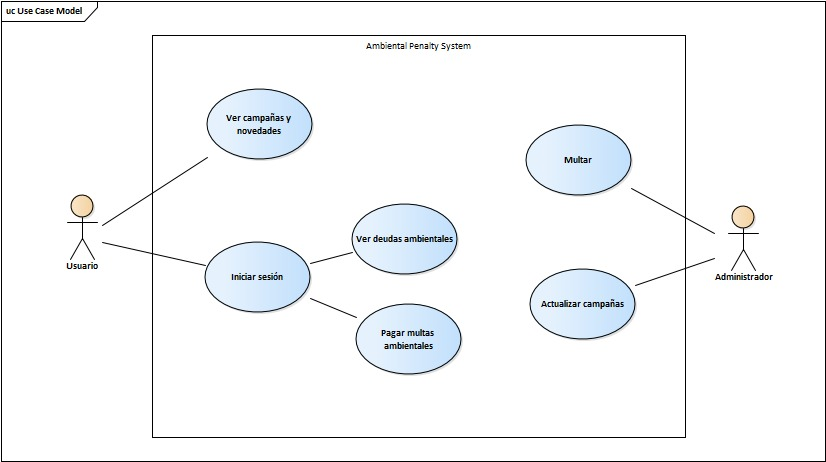
\includegraphics[scale=0.5]{DIAGRAMuSOS.jpg} 
\end{center}

\begin{center}
\textbf{\Large DIAGRAMA DE CLASES\\}
\end{center}
\begin{center}
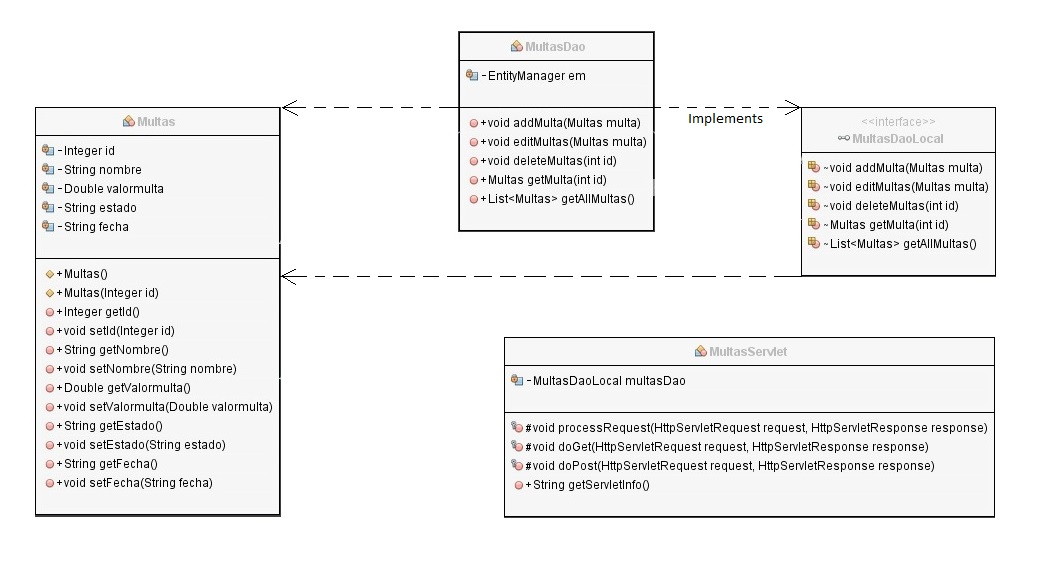
\includegraphics[scale=0.5]{DIAGRAMcLASES.jpg}  
\end{center}

\begin{center}
\textbf{\Large DIAGRAMA DE DESPLIEGUE\\}
\end{center}
\begin{center}
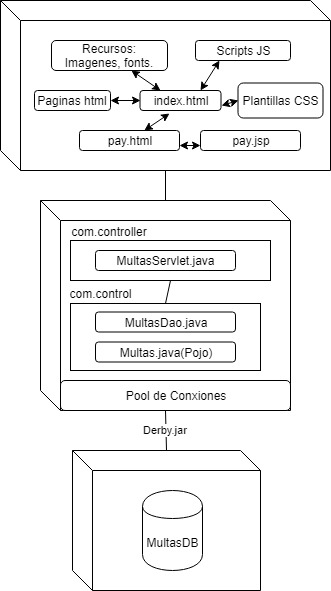
\includegraphics[scale=0.8]{DIAGRAMdES.jpg} 
\end{center}
}
\thispagestyle{empty}
$ $
\end{document}

